\chapter{Design}
After analyzing the problem, this chapter will go through the design of the application architecture of our UIProtocol client. The design phase is of crucial importance as it is the time when important design decisions are made. In this phase, the application's architecture needs to be thought through so that its future extensions are relatively easy to implement and cost of maintenance is low.\\
From the analysis we will conclude requirements for the application which will be developed. Further on, the sections will describe the design of several sub-systems which are responsible for handling the communication, models, events, inner representation of the UI elements, their rendering and more.\\
Even though there are existing implementations of UIProtocol client, the design of this one was not influenced by any of them.

\subsection{Requirements}
The client application will be developed and run on Windows Phone 8 device. Since the entire user interfaces and information about events is intended to be transferred over wireless internet connection, there will be a delay present in the application's reaction time, which is a inescapable consequence of the client-server architecture. The delay should be reasonably small to allow for a comfortable usage of the application. Even with this delay, the application should perform well in terms of UI rendering times, reaction time and overall feel.\\
There is a number of requirements an app should meet in order to be truly accessible. In our analysis, we found that the support of Windows Phone 8 for accessibility is lower than at the competing platforms. Namely, support for a key accessibility feature, a screen reader, is not present by default. This holds true even for the Windows Phone 8.1 which was released in February 2014. This can be a major flaw to the application accessibility – especially for visually impaired who would have to use a third-party screen reader in order to be able to navigate through the app. Apart from following the guidelines for developing accessible apps, as discussed in \ref{sec:accGuidelines}, we may propose some new features that could be implemented by UIProtocol to increase its own support for accessibility. At any rate, even with the Windows Phone 8 platform's low accessibility support, the developed app will remain a fully functional UIP client capable of displaying valid UIP documents.


\subsubsection{Summary of Requirements}
From the requirements section, we have developed the following lists of non-functional and functional requirements, respectively.
\\
Non-functional requirements:
\begin{itemize}
  \item UI components have platform native look
  \item App will be will be written in C\#
  \item The client should not use much phone resources when idle
  \item App should be stable and able to process valid UIP documents
  \item Compatibility with UIP standard, draft 8
  \item Ability to run on any WP8 device
  \item UI loading times below 0.5 s with stable internet connections
\end{itemize}
~\\
Functional requirements:
\begin{itemize}
  \item  Support for basic user interface elements
  \item Graceful degradation for unsupported elements
  \item  Support for binding and model-wide binding
  \item  Support for interpolated model updates (animations)
  \item  Support for UI generator API
  \item Support for absolute and grid layouts
  \item Support for styling (font size, colors, etc.)
\end{itemize}

\subsection{Client-server Communication}
The client will communicate with the server over TCP-IP connection which will be handled by a standard socket. Upon this communication channel, UIProtocol XML files will be transferred.\\
Once the client connects to the server and goes through the connection procedure described in \cite{uip}, the server sends the XMLs describing the UI. The UML diagram of the classes responsible for the communication is shown in figure \ref{fig:classComm}. Since some of the methods will only work with the passed parameters and not modify the object's state, they will be made static. 

\begin{figure}[ht!]
\centering
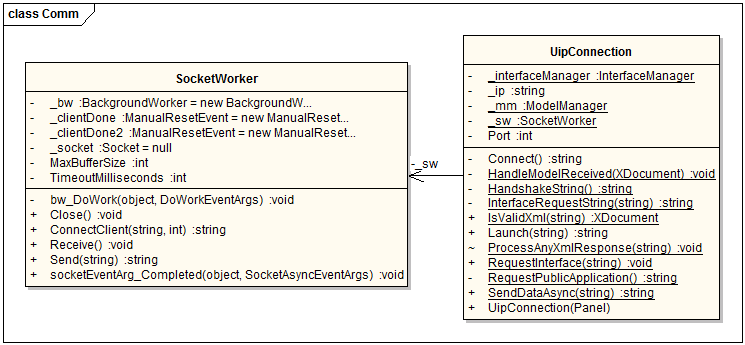
\includegraphics[width=145mm]{pics/3/classComm.png}
\caption{Inheritance tree of several sample UI classes}
\label{fig:classComm}
\end{figure}

Apart from the mentioned classes that will serve for communicating the XML messages, there there will be another class responsible for acquiring resources (such as images) from the server. For this purpose, the server is awaiting a connection on another port than the XML server <-tohle lepe posat TODO and the client can open a connection and make a standard http request for the resource. This functionality will be implemented in the TcpConncetion class.

\subsection{Parsing XML Into Inner Object Representation}
After the UIP documents will be received by the UipConnection class, they will be passed to instances of ModelManager and InterfaceManager classes. ModelManager will be responsible for processing possible new models or model updates and will be discussed later in more detail.\\
All of the UIP elements need to be represented by objects, so that 
The InterfaceManager class will process the XML data that describes the UI by recursively traversing the XML tree and creating instances of Interface, Container and Element classes, based on the type of the considered XML node. These instances will represent the UIP elements of the same name - UIP interface, UIP container and UIP element. This way, every UIP element will be parsed into an inner object representation that will be easy to handle when in further work with the objects.

\begin{figure}[ht!]
\centering
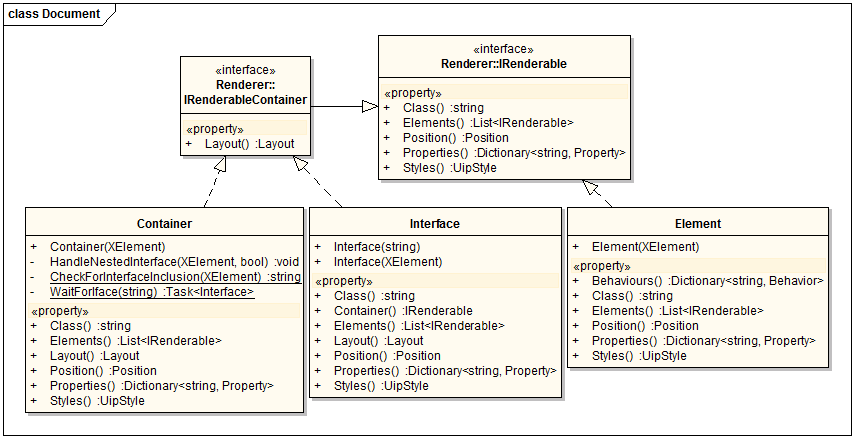
\includegraphics[width=145mm]{pics/3/classDocument.png}
\caption{document class diagram}
\label{fig:classDocument}
\end{figure}

An important component is the IRenderable interface from whom the Interface, Container and Element classes inherit. This interface represents the functionality all of the classes have in common - most importantly the UIP class (i.e. type of the UI control - see todo), UIP properties and contained elements. IRenderableContainer only extends the IRenderable interface by adding a method for obtaining a layout. Since layout is a container feature, only Interface and Container classes will inherit from it.

\subsection{Managing Models and Binding}
The client, to conform the UIP specification must be a thin client, i.e. it will only store as much data as is needed to render the required interfaces and not execute any code on that data. The data shown to the user can be either constant or come from models, which are designed as a data storage. Models will be managed by one instance of ModelManager class.\\
If an UIP element has a property that refers to a model, ModelManager will be responsible for requesting the model containing this property. Once the model is received, ModelManager will store all its properties and will manage future model updates. Note that the updates can come from the server at any time. ModelManager will also contain <zlepsit TODO> a reference to InterfaceManager because server's models can contain a request to render an interface. The relationship between classes that are involved in Model management is shown in figure \ref{fig:classModel}.
\\
todo binding
\\
\begin{figure}[ht!]
\centering
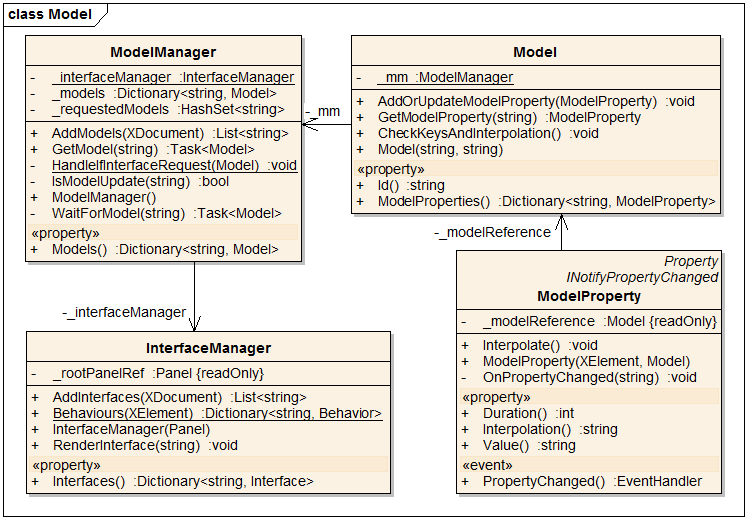
\includegraphics[width=145mm]{pics/3/classModel.png}
\caption{models class diagram (simplified)}
\label{fig:classModel}
\end{figure}


\subsection{Managing Interfaces}
Interface is the root element for all UI controls in UIP documents. An application can contain a large number of interfaces. We therefore need a class to keep all the information. InterfaceManager will serve as a place for storing information about received and requested interfaces. The most important methods implemented in it will be for adding received interfaces, obtaining an interface and rendering. The process of rendering is described more closely in the next section.

\subsection{Rendering the UI}
After the received XML description of the user interface is processed, InterfaceManager calls the Render() method of the Renderer class. This method traverses the tree of the newly created instances of classes from figure \ref{fig:classDocument} and for each one creates a wrapper class which inherits from UipBase. 

\begin{figure}[ht!]
\centering
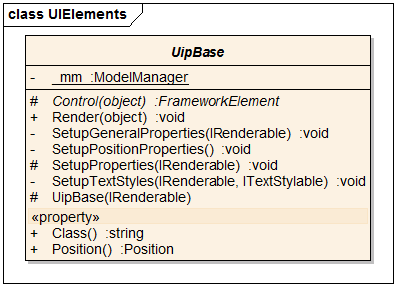
\includegraphics[width=70mm]{pics/3/classUipBase.png}
\caption{UipBase class diagram}
\label{fig:classUipBase}
\end{figure}


\subsection{Representing the Platform-native UI Components}
In order to support easy addition of the supported UI elements, we created classes shown in figure todo. There is an abstract base class, UipBase which contains methods for model updates, styling and element dimensions.\\
Any particular UI element needs to inherit from the base class in order to support rendering, model updates and other functionality provided by the base class.

\subsection{Events}
The application is designed to support the client-to-server communication in form of events. Events are the only data sent by the client and their intent is to inform server of an user action or request missing data - models.\\

Events could be divided into two categories.\\
Events that are static and are hard-coded within the application. These events are used rarely, typically while going through the procedure of connecting to the server. Currently these are the "public.connection.connect" and "public.request.model" request for "public.application".
Other events are the ones triggered by the user or by the client itself, when it requests a model. These events are dynamic, created at runtime. The event firing - e.g. notifying server of an action taking place, is a relatively simple process which will be handled by two classes.\\
EventManager: the class's only task is to provide a method for sending an event. The class won't contain any state and will therefore be static, which will make it easily accessible from any point of the application. Its job will be to merely forward the events to SocketWorker class instance which will do the actual job of sending them to the server.\\
Event class will represent a particular event that will be sent to the server. It will contain all the necessary information for the server to be able to identify the event that has been triggered, as specified in todo. This information will be stored in properties.

\begin{figure}[ht!]
\centering
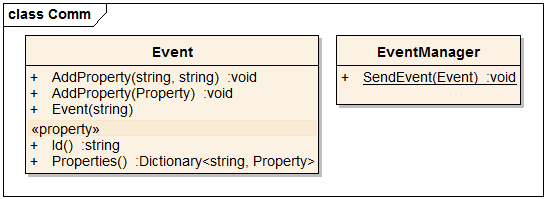
\includegraphics[width=130mm]{pics/3/classEvent.png}
\caption{event class diagram}
\label{fig:classEvent}
\end{figure}

\subsection{Properties}
Properties are the most nested objects in UIP documents. They are used extensively within many classes, including Layout, Event or Element. In all classes they will be stored in dictionaries, identified by their name.

The ModelProperty class used in Model will inherit from Property class. They are directly attached to the particular class instance.

\subsection{Layouts}
... Two layout types will be supported in our client: absolute and grid. Even though absolute layout is not recommended by the accessibility guidelines ref todo it is a basic form of layout and decision has been made to support it.
Layouts are a feature of containers and interfaces which support it through the I render able container interface. Every container, therefore can place its content into one of the two. As with any property, the positioning will be Bindable. The laYout is represented by the layout class. Haha obvious.

\subsection{Configuration}
Client will have support for basic co figuration- I.e. ports on which the socket is tying to connect. Also the constants which are used in the portions of XML throughout the application will be stored in one static class so that they are easy to change. 

\subsection{Behaviors}
Behaviors are used to attach event listeners to UI controls. C\# has a built-in support for events through Event and Delegate classes and we will take advantage of it.\\
Behaviors will be attached to the classes inheriting from UipBase as event handlers. Each handler is for one type of behavior 

%\begin{figure}[ht!]
%\centering
%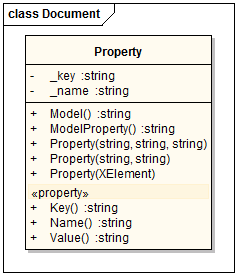
\includegraphics[width=60mm]{pics/3/classProperty.png}
%\caption{properties class diagram}
%\label{fig:classProperty}
%\end{figure}

behavior, layouts, positions, settings, interpolace
